\subsection{Class Diagram}


The main structure of the class diagram is divided into two parts, one is for the filter package, while the other is for the Servelet package. 
For the filter package shown at the left bottom of the diagram, the class diagram is relatively easy to read. LoginFilter class 'extends' the AbstractFilter class.
For the rest of the classes, there are twelve resources to handle from analytics to user. Among those resources, Activities, Template, and Analytics are using 
a single servlet to implement CRUL queries, while others employ the REST paradigm. Specifically, to compare and contrast the TemplateSerevelt and 
UserRestResource to understand the whole picture of the class diagram. 
Concerning the user, there are multiple servlets used to handle the user
resource. In particular, we have a servlet (UserServlet) that is mapped to URIs that are freely accessible from
outside.\\

In the case of Template, it uses a servlet (TemplateServlet) to handle the template
resource. In the TemplateServlet, it utilizes DoGet, DoPost, and DoDelete provided by
Class HttpServlet to get, delete, update, and insert template. TemplateServlet also has several subclasses, for instance, it overrides the
method “DeletionOperations” to delete the template by the template id. In this subclass, it calls the Data Access Objects (DAOs), 
DeleteTemplateDatabase, to access data in the database. Note that TemplateServlet
has been kept mainly for legacy reasons.\\

Concerning the User, the servlet that implements the required behaviors to handle such resources is a more traditional servlet, based on the
REST paradigm. In particular, we have a servlet, which also handles the Users resource, and parses the
URI determines the type (and possibly the id) of the resource that the user wants to interact with. Once the
servlet has processed the request, it forwards it to the proper Rest Manager class. There are six rest manager
classes including UserRestResource, which is a sub-classes of RestResource and implement the
methods to handle the proper resource.\\
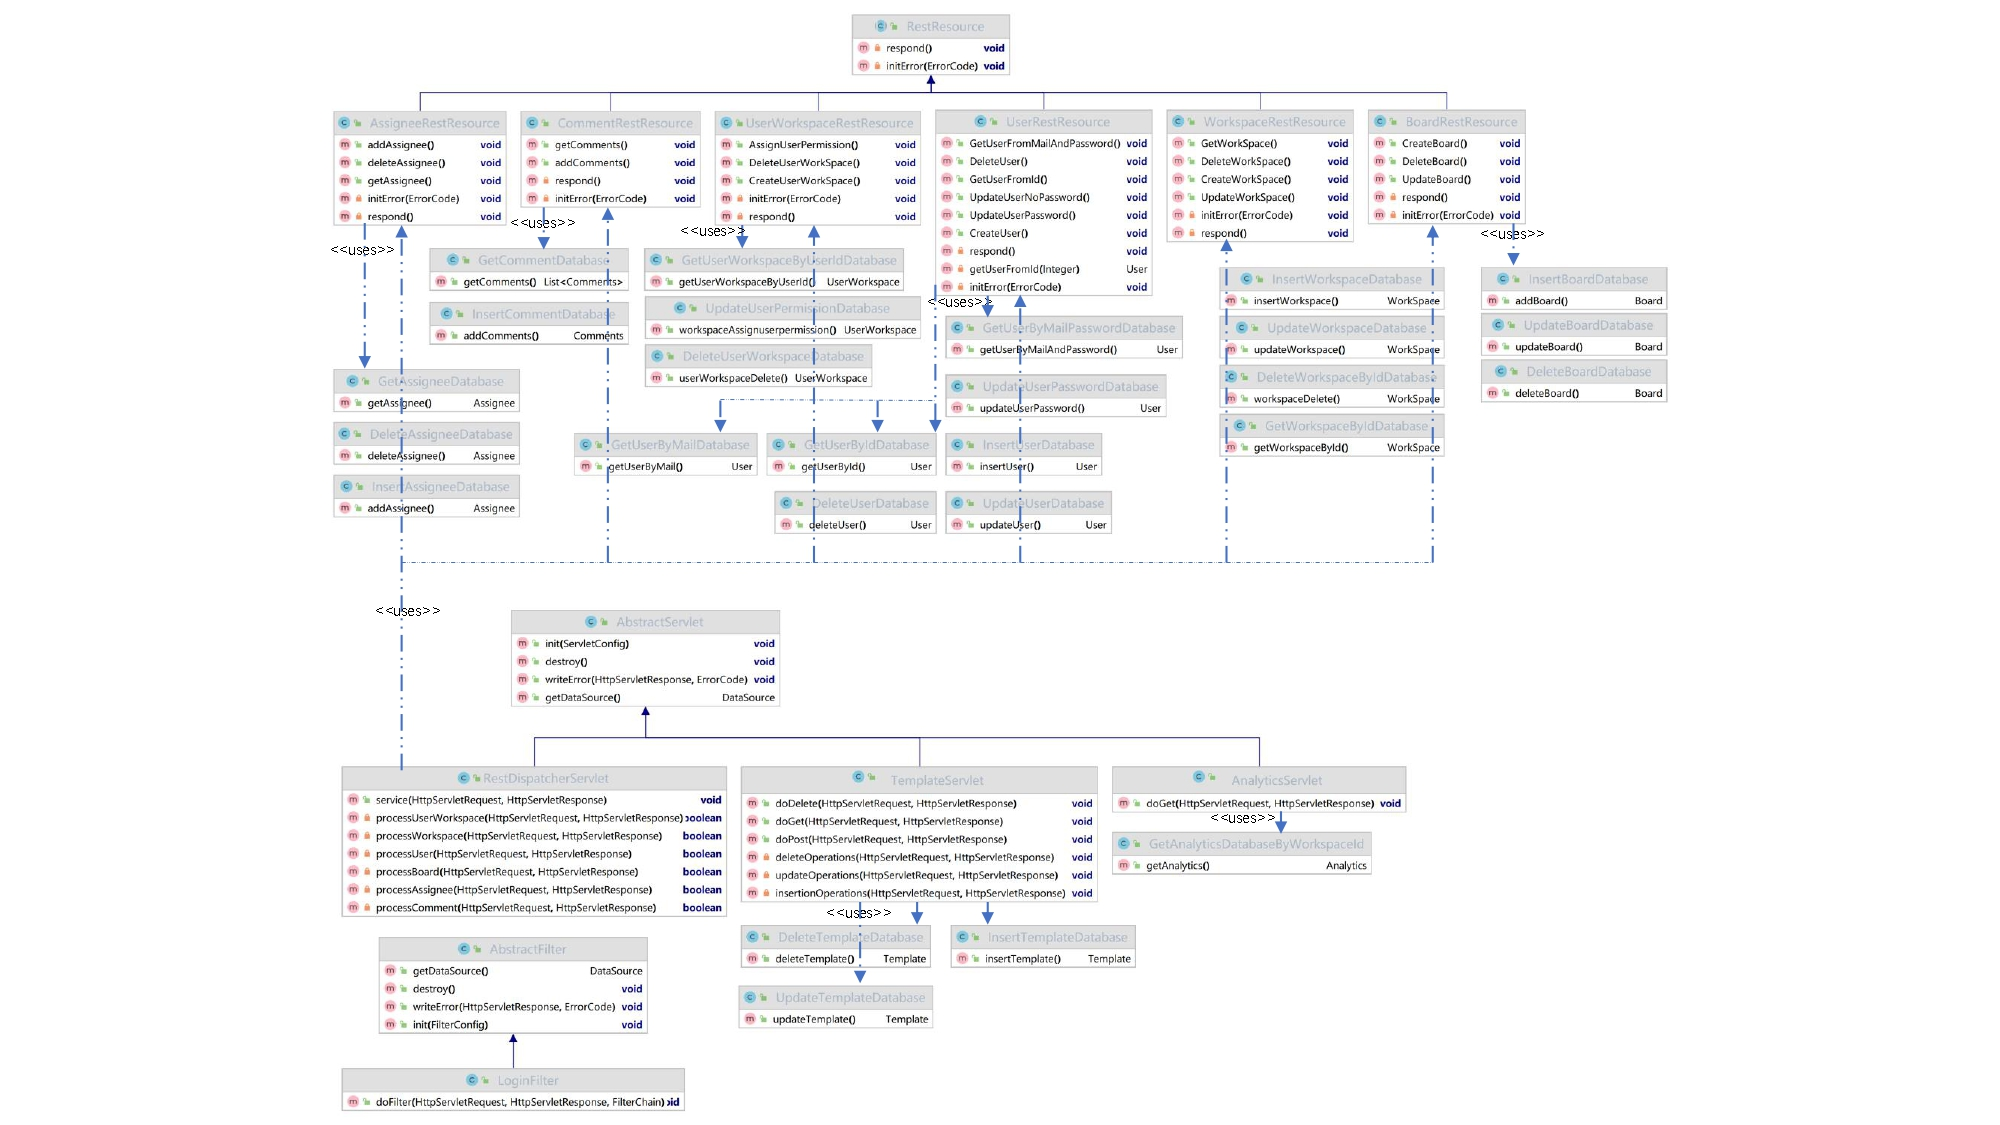
\includegraphics[width=1.30\columnwidth]{WA-workflix-HW1/images/class sequence.jpg}\\

\subsection{Sequence Diagram}
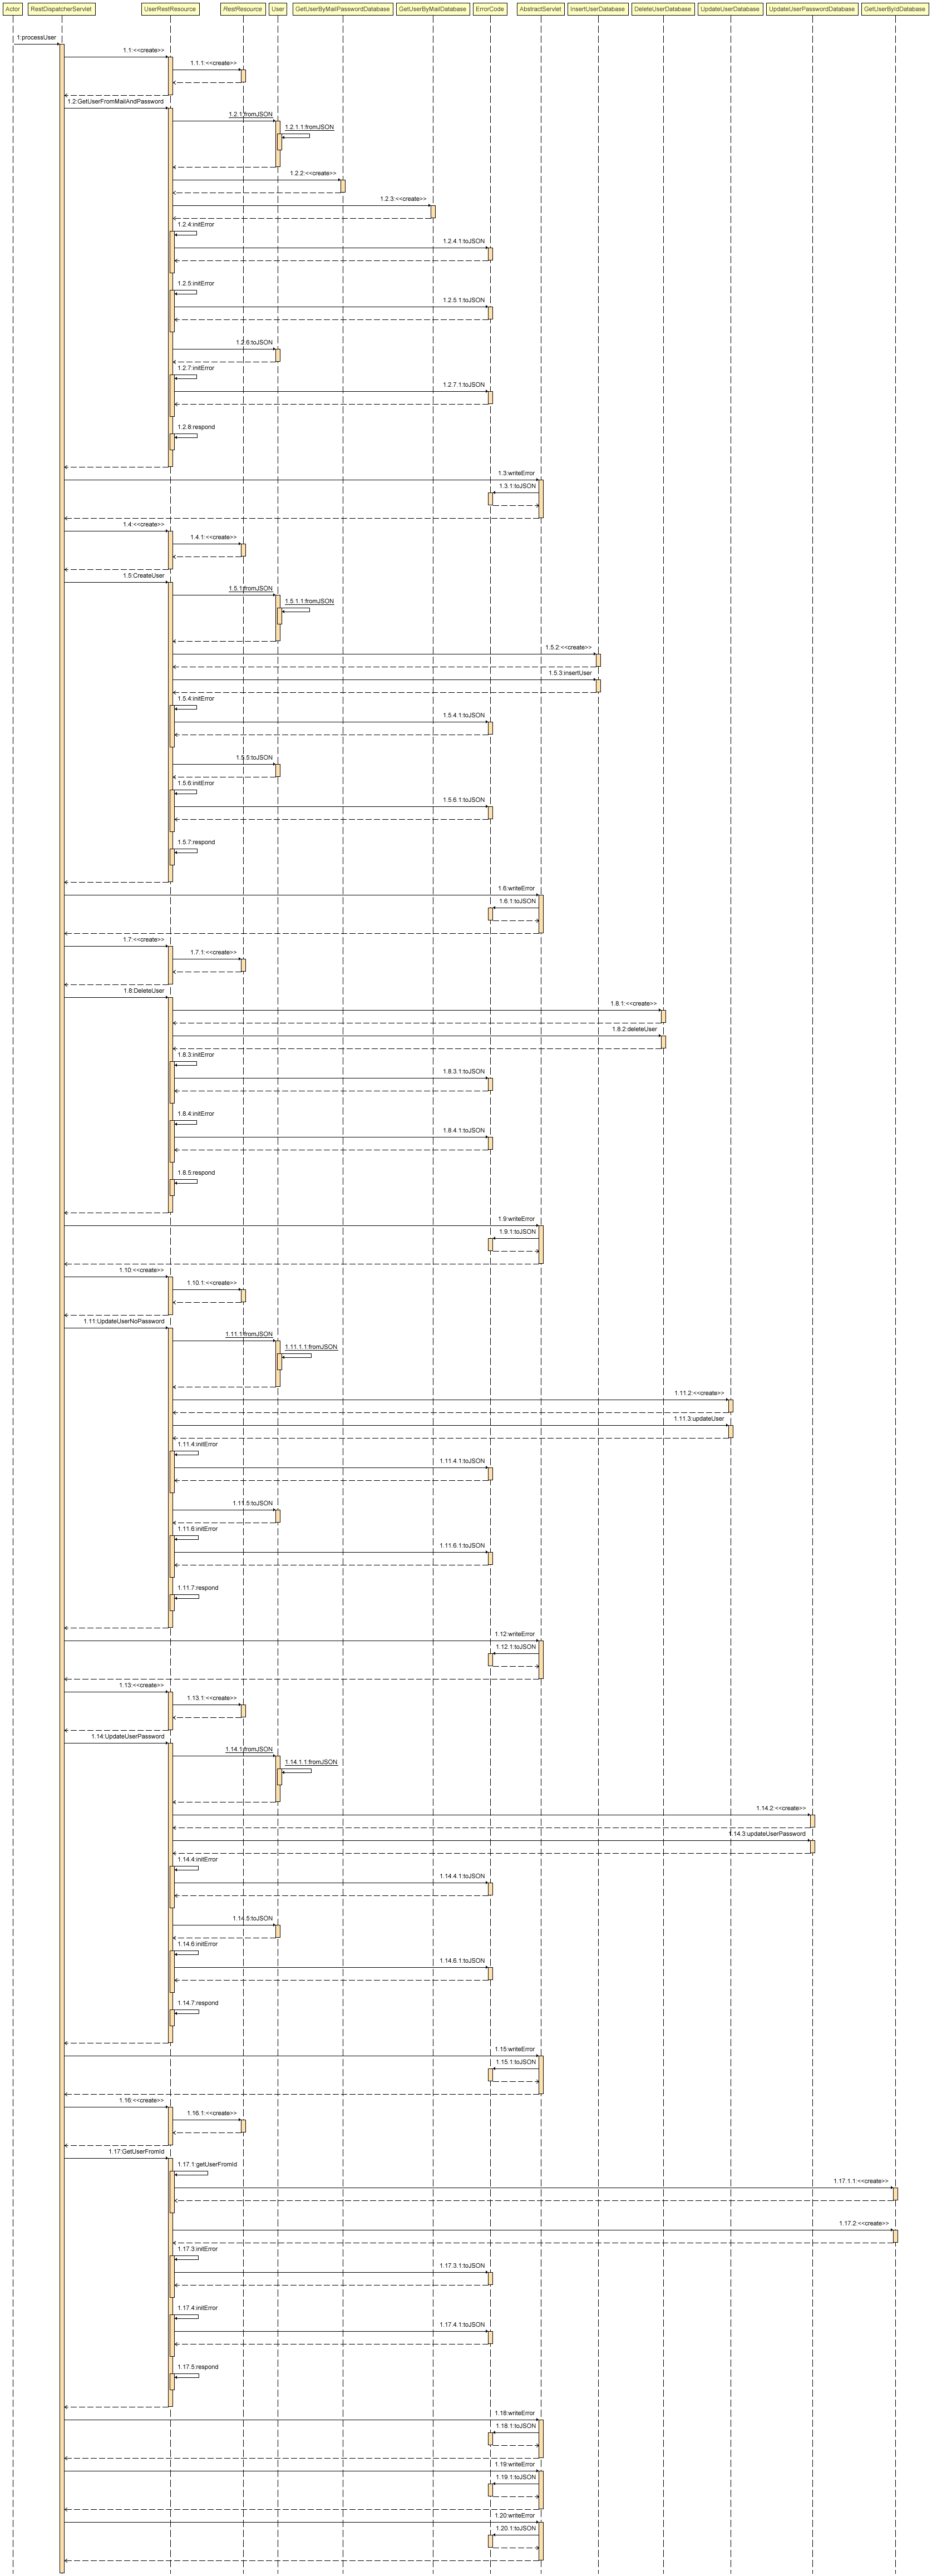
\includegraphics[width=0.5\columnwidth]{WA-workflix-HW1/images/RestDispatcherServlet_processUser.jpg}